\documentclass[utf8, a4paper]{beamer}
%\documentclass[pdf]{beamer}
\mode<presentation>{\usetheme{Frankfurt}}

%\usepackage[utf8x]{inputenc} % in order to use "à" like symbols
\usepackage{xparse}
\usepackage{xspace}
\usepackage{graphicx}
\usepackage{tikz}
\usepackage{hyperref}
\usepackage{bm}
\usepackage{caption}
\usepackage{subcaption}
\usepackage{phdGeneral}
\usetikzlibrary{matrix} %to use matrices in tikz pictures (https://tex.stackexchange.com/a/126974/145331)
\usetikzlibrary{arrows.meta} %to customize arrows in tikz
\usetikzlibrary{arrows}


\NewDocumentCommand{\tuple}{m}{%
	\nmath{\langle{#1}\rangle}%
}

\NewDocumentCommand{\induced}{m m}{%
	\nmath{I(#1, #2)}%
}

\NewDocumentCommand{\set}{m}{%
	\nmath{\{#1\}}%
}

\NewDocumentCommand{\code}{m}{%
	\texttt{#1}%
}


%%%%%%%%%%%%%%%%%%%%%%%%% ALIAS %%%%%%%%%%%%%%%%%%

\NewDocumentCommand{\subgraphvar}{}{%
	\nmath{\mathscr{F}}%
}

\NewDocumentCommand{\sccsubsetvar}{m}{%
	\nmath{S}_{#1}%
}

\NewDocumentCommand{\true}{}{%
	\texttt{true}%
}

\NewDocumentCommand{\false}{}{%
	\texttt{false}%
}

\NewDocumentCommand{\graph}{}{%
	\nmath{\mathcal{G}}%
}

\NewDocumentCommand{\epoch}{}{%
	\nmath{\rho}%
}

\NewDocumentCommand{\chain}{O{\csp{}}}{%
	\nmath{\mathcal{C}(#1)}%
}

\newcommand{\noteq}{\nmath{\not =}}

\NewDocumentCommand{\fsccs}{}{%
	\nmath{S}%
}

\NewDocumentCommand{\elt}{O{\scc{}}}{%
	\nmath{E_{<}[#1]}%
}

\NewDocumentCommand{\eneq}{O{\scc{}}}{%
	\nmath{E_{\not =}[#1]}%
}

\NewDocumentCommand{\fscc}{}{%
	\nmath{\sigma_{\texttt{flawed}}}%
}

\NewDocumentCommand{\scc}{}{%
	\nmath{\sigma}%
}

\NewDocumentCommand{\csp}{}{%
	\nmath{\Theta}%
}

\NewDocumentCommand{\IACSP}{}{%
	\nmath{\Omega}%
}

\NewDocumentCommand{\piOne}{O{\IACSP{}}}{%
	\nmath{\pi_{1}(#1)}%
}

\NewDocumentCommand{\piTwo}{O{\IACSP{}}}{%
	\nmath{\pi_{2}(#1)}%
}

\NewDocumentCommand{\SigmaOne}{}{%
	\nmath{\Sigma_1}%
}

\NewDocumentCommand{\SigmaTwo}{}{%
	\nmath{\Sigma_2}%
}

\NewDocumentCommand{\edge}{m m m}{%
	\nmath{(}#1\nmath{, }#2\nmath{, }#3\nmath{)}%
}

\NewDocumentCommand{\tlGraph}{}{%
	TL-Graph%
}

\NewDocumentCommand{\DPASAT}{}{%
	\textsc{Dpasat}%
}

\NewDocumentCommand{\DOHSAT}{}{%
	\textsc{Dohsat}%
}


\NewDocumentCommand{\OHSAT}{}{%
	\textsc{OrdHorn-SAT}%
}

\NewDocumentCommand{\PC}{}{%
	\textsc{PC}%
}

\NewDocumentCommand{\dpsat}{}{%
	\texttt{D-PSAT}%
}

\NewDocumentCommand{\disat}{}{%
	\texttt{D-ISAT}%
}

\NewDocumentCommand{\conv}{m}{${#1}^{\smile}$}

\NewDocumentCommand{\iab}{}{%
	{\sf b}%
}

\NewDocumentCommand{\iabi}{}{%
	\conv{\sf b}%
}

\NewDocumentCommand{\iam}{}{%
	{\sf m}%
}

\NewDocumentCommand{\iami}{}{%
	\conv{\sf m}%
}

\NewDocumentCommand{\iad}{}{%
	{\sf d}%
}

\NewDocumentCommand{\iadi}{}{%
	\conv{\sf d}%
}

\NewDocumentCommand{\ias}{}{%
	{\sf s}%
}

\NewDocumentCommand{\iasi}{}{%
	\conv{\sf s}%
}

\NewDocumentCommand{\iaf}{}{%
	{\sf f}%
}

\NewDocumentCommand{\iafi}{}{%
	\conv{\sf f}%
}

\NewDocumentCommand{\iao}{}{%
	{\sf o}%
}

\NewDocumentCommand{\iaoi}{}{%
	\conv{\sf o}%
}

\NewDocumentCommand{\iaeq}{}{%
	{\sf $=$}%
}


%\NewDocumentCommand{\code}{m}{\texttt{#1}}
%\NewDocumentCommand{\CSP}{O{\Theta}}{#1}
%\NewDocumentCommand{\noteq}{}{\not =}
%\NewDocumentCommand{\tuple}{m}{(#1)}
%\NewDocumentCommand{\psat}{}{\textsc{PSAT}}
%\NewDocumentCommand{\dpsat}{}{\textsc{D-PSAT}}
%\NewDocumentCommand{\disat}{}{\textsc{D-ISAT}}
%\NewDocumentCommand{\isat}{}{\textsc{ISAT}}
\NewDocumentCommand{\nphard}{}{\textsc{NP-Hard}}
\NewDocumentCommand{\dpasat}{}{\textsc{DPASAT}}
%\NewDocumentCommand{\dohsat}{}{\textsc{DOHSAT}}
\NewDocumentCommand{\ohsat}{}{\textsc{OHSAT}}
%\NewDocumentCommand{\TLGraph}{}{TL\--\-Graph}
%\NewDocumentCommand{\sccvar}{}{\sigma}
%\NewDocumentCommand{\msQuote}{m}{`#1`}
\NewDocumentCommand{\mdQuote}{m}{``#1''}
%\NewDocumentCommand{\conv}{m}{{#1}^{\smile}}

%\NewDocumentCommand{\EdgeSet}{o m}{%
%	\IfNoValueTF{#1}{%
%		E_{#2}
%	}{%
%		E_{#2}\left[#1\right]
%	}
%}



%\newenvironment<>{varblock}[2][\textwidth]{%
%	\setlength{\textwidth}{#1}%
%	\begin{actionenv}#3%
%		\def\insertblocktitle{#2}%
%		\par%
%		\usebeamertemplate{block begin}%
%	}{\par%
%		\usebeamertemplate{block end}%
%\end{actionenv}%
%}

\NewDocumentCommand{\TheTitle}{}{Efficient Algorithms for Graph-Based Knowledge Bases}
\NewDocumentCommand{\TheAuthor}{}{Massimo Bono}

%THEME

%\usetheme{progressbar}
%\progressbaroptions{
%	headimage=img/logo_big.png,
%	titleimage=img/logo2.png,
%	blocks/width=0.98\textwidth,
%}
%edit the footer of the slides
\makeatother
\setbeamertemplate{footline}
{
	\leavevmode%
	\hbox{%
		\begin{beamercolorbox}[wd=.3\paperwidth,ht=2.25ex,dp=1ex,center]{author in head/foot}%
			\usebeamerfont{author in head/foot}\TheAuthor{}
		\end{beamercolorbox}%
		\begin{beamercolorbox}[wd=.7\paperwidth,ht=2.25ex,dp=1ex,center]{title in head/foot}%
			\usebeamerfont{title in head/foot}\TheTitle{}\hspace*{3em}
			\insertframenumber{} / \inserttotalframenumber\hspace*{1ex}
	\end{beamercolorbox}}%
	\vskip0pt%
}
\makeatletter
\setbeamertemplate{navigation symbols}{}
\setbeamersize{text margin left=1em, text margin right=1em}

%END THEME

\graphicspath{{img/}}

\title{\TheTitle{}}
\author{%
	{\TheAuthor{}}\\%
	{Tutor: Alfonso Emilio Gerevini}\\%
	{XXXII cycle, \mdQuote{Ingegneria Informatica ed Automatica} Curriculum}\\%
	{email: \code{mbono@unibs.it}}\\%
	\vspace{0.3cm}%
	
\includegraphics[width=0.2\textwidth]{logo_big}\\%
}
%\date{\today}

\addSrcFolder{{src/texs/}}
\addSrcFolder{{src/tikzs/}}
\addImagesFolder{{src/imgs/}}

\begin{document}
	
%TITLE PAGE
{
	\setbeamertemplate{footline}{} 
	\begin{frame}[plain]
		\titlepage
	\end{frame}
}


\section{Introduction}

\subsection{}
\begin{frame}{Outline}
	\begin{enumerate}
		\item Decremental Consistency Checking Problem:
			\begin{itemize}
				\item Background;
				\item proposed techniques;
				\item experimental results.
			\end{itemize}
		\item Dynamic Path Planning:
			\begin{itemize}
				\item Background;
				\item proposed techniques;
				\item preliminary results.
			\end{itemize}
		\item Conclusions and future works.
	\end{enumerate}
\end{frame}

\section{Decremental Consistency Checking Problem}

\subsection{}
\begin{frame}{The problem with a motivating example}
	\begin{figure}
		\centering
		\begin{subfigure}{0.5\textwidth}%
			\includeTikz{touristExample.ia.before.6}[0.6]%
		\end{subfigure}\hfill%
		\begin{subfigure}{0.5\textwidth}%
			\includeTikz{touristExample.ia.before.6.solution}[0.6]%
		\end{subfigure}%
%		\begin{subfigure}{0.01\textwidth}%
%			\includegraphics[width=.5\textwidth, angle=270]{graph.ps}
%		\end{subfigure}
	\end{figure}
	
\end{frame}

\subsection{}
\begin{frame}{Background}
	\begin{block}{Constraint Satisfactory Problem}%
		A CSP $\csp{}$ involves a set of $n$ \textit{variables} $X_1, X_2, ... X_n$ having domains $D_1, D_2, ..., D_n$ where each $D_i$ defines the set of values the variable $X_i$ may assume. CSPs may have n-ary \textit{constraints} $R$ s.t. $R \subseteq D_1 \times D_2 \times ..., D_n$. 
	\end{block}
	
	\begin{itemize}
		\item We focus on temporal CSPs;
		\item Domains: time points/interval;
		\item Constraints: Point Algebra, Ord-Horn Subalgebra, Interval Algebra;
	\end{itemize}
	
	\begin{table}
		\centering
		\begin{tabular}{c|c}
			\textbf{base relations}		&	\textbf{resulting relation} \\ \hline
			$\emptyset$			&	$\bot$	\\
			$<$					&	$<$		\\
			$=$					&	$=$		\\
			$>$					&	$>$		\\
			$< \cup =$			&	$\leq$	\\
			$< \cup >$			&	$\noteq$\\
			$= \cup >$			&	$\geq$	\\
			$< \cup = \cup >$	&	$\top$	\\
		\end{tabular}
	\end{table}
\end{frame}

\subsection{}
\begin{frame}{Background}
	\begin{block}{Consistency}
		A CSP $\csp{}$ is \textbf{consistent} iff there is at least one solution (\ie{} assignment of values to all the variables $\{X_i = v_i\}$ s.t. no constraint is violated).
	\end{block}
	
	\begin{block}{\tlGraph{}}
		Graph $\mathcal{G} = (V, E)$ where each vertex in $V$ represents a CSP variable, each edge in $E$ represents a PA constraint in the CSP. Edges are either directed and labeled as \sQuote{$\leq$} or \sQuote{$<$}, or undirected and labeled as \sQuote{$\not =$}.
	\end{block}
	
	Given:
	\begin{itemize}
		\item[-] \small{an \textbf{inconsistent temporal CSP} \csp{} over a class of constraints
$\cal C$};
		\item[-] \small{a \textbf{sequence $\bm{\csp{}_{0}, ..., \csp{}_k}$ of CSPs} over $\cal C$ such that $\csp{}= \csp{}_{0}$ and $\csp{}_i$ is obtained from $\csp{}_{i-1}$ by making one constraint relaxation in $\csp{}_{i-1}$, for $i = 1, ..., k$};
	\end{itemize}
	\textbf{\color{blue} Decremental Consistency Checking} is the problem of \textit{iteratively deciding the consistency} of every $\csp{}_i$ starting from $\csp{}_1$ until $i = k$ or $\csp{}_i$ becomes consistent.
\end{frame}

\subsection{}
\begin{frame}{How to solve the Decremental Consistency Checking Problem?}
	For PA:
	\begin{itemize}
		\item van Beek algorithm ($O(v+e)$);
		\item \dpasat{}: decremental version of van Beek algorithm; compute useful metadata once and repair them only when strictly needed.
	\end{itemize}
	For Ord-Horn subalgebra:
	\begin{itemize}
		\item Path Consistency ($O(n^3)$) or \OHSAT{} ($O(c \dot n)$);
		\item \DOHSAT{}: decremental version of \OHSAT{};
	\end{itemize}
\end{frame}

\subsection{}
\begin{frame}{Experimental Results}
	\begin{figure}
		\centering
		\begin{subfigure}{0.5\textwidth}%
			\includegraphics[width=1.0\textwidth]{{{a1.SPARSE.RELAXALL.REFSCC.meantimes.given.size.logy.linearx}}}%
		\end{subfigure}\hfill%
		\begin{subfigure}{0.5\textwidth}%
			\includegraphics[width=1.0\textwidth]{{{a1.SPARSE.RELAXALL.ALLRELATIONS_RANDOM_meantimes_given_size_logy_linearx}}}%
		\end{subfigure}%
	\end{figure}
\end{frame}

\section{Path Planning}

\subsection{}
\begin{frame}{Path Planning: the problem and a motivating example}
	\begin{figure}
		\centering
		\includegraphics[width=0.45\textwidth]{{{paths}}}
		\caption{Source: XKCD at \url{https://xkcd.com/85/}}
	\end{figure}
\end{frame}

\subsection{}
\begin{frame}{Background}
	\begin{definition}{Compressed Path Database (CPD)}
		Data structure compactly representing, for each cell in the the map, the first optimal move to perform in order to reach a target location.
	\end{definition}
	
	\begin{minipage}{0.5\textwidth}
		High level view: 
		\begin{itemize}
			\item run Dijkstra from every location in the grid as starting point (storing only the first move);
			\item compress the result.
		\end{itemize}
	\end{minipage}%
	\begin{minipage}{0.5\textwidth}
			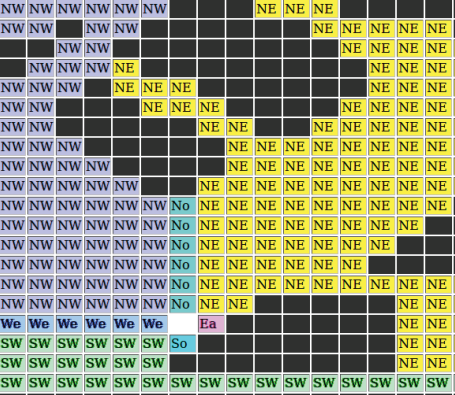
\includegraphics[width=0.95\textwidth]{gridmap}
	\end{minipage}
\end{frame}

\subsection{}
\begin{frame}{How to repair the path once a perturbation occured?}
	\begin{block}{Main idea}
		Use A* algorithm where the heuristic is the cost of the optimal path in the original map. We stop the search when:
		\begin{itemize}
			\item we find the goal;
			\item the path generated by the CPD is clear from perturbations;
		\end{itemize}
	\end{block}
	
	\begin{figure}
		\centering
		\begin{subfigure}{0.45\textwidth}
			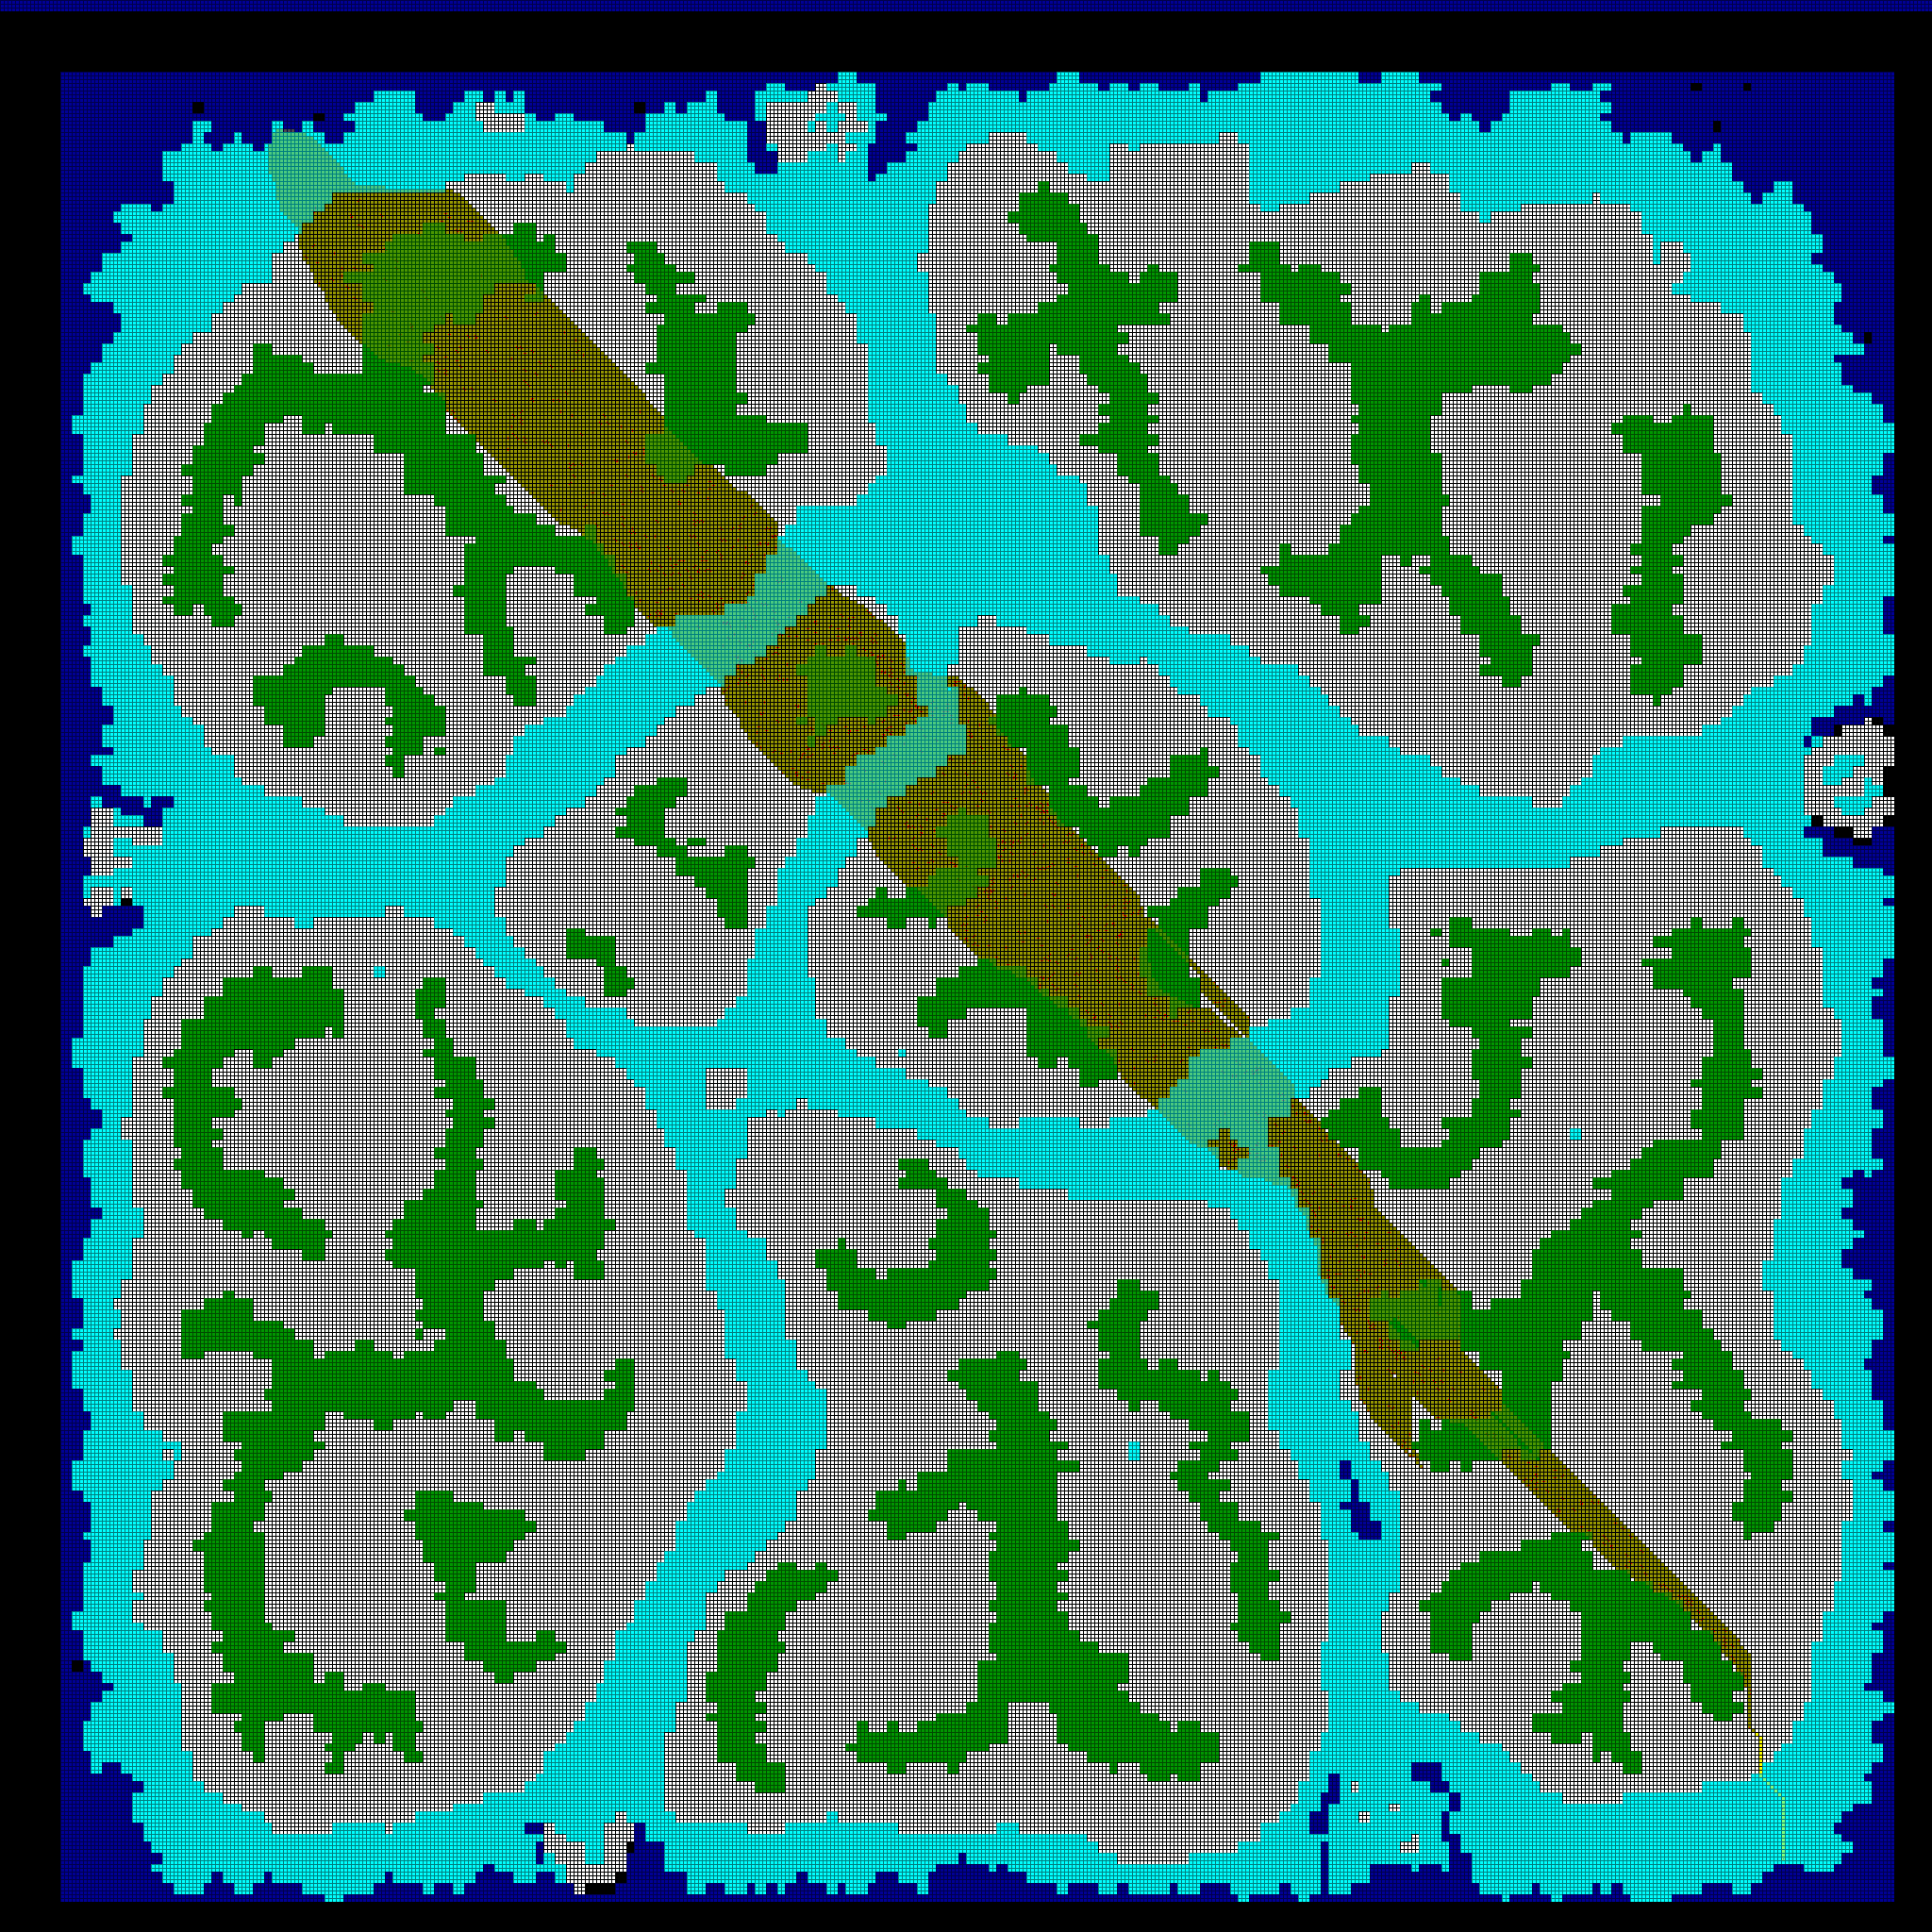
\includegraphics[width=0.8\textwidth]{Astar}
		\end{subfigure}\hfill%
		\begin{subfigure}{0.45\textwidth}
			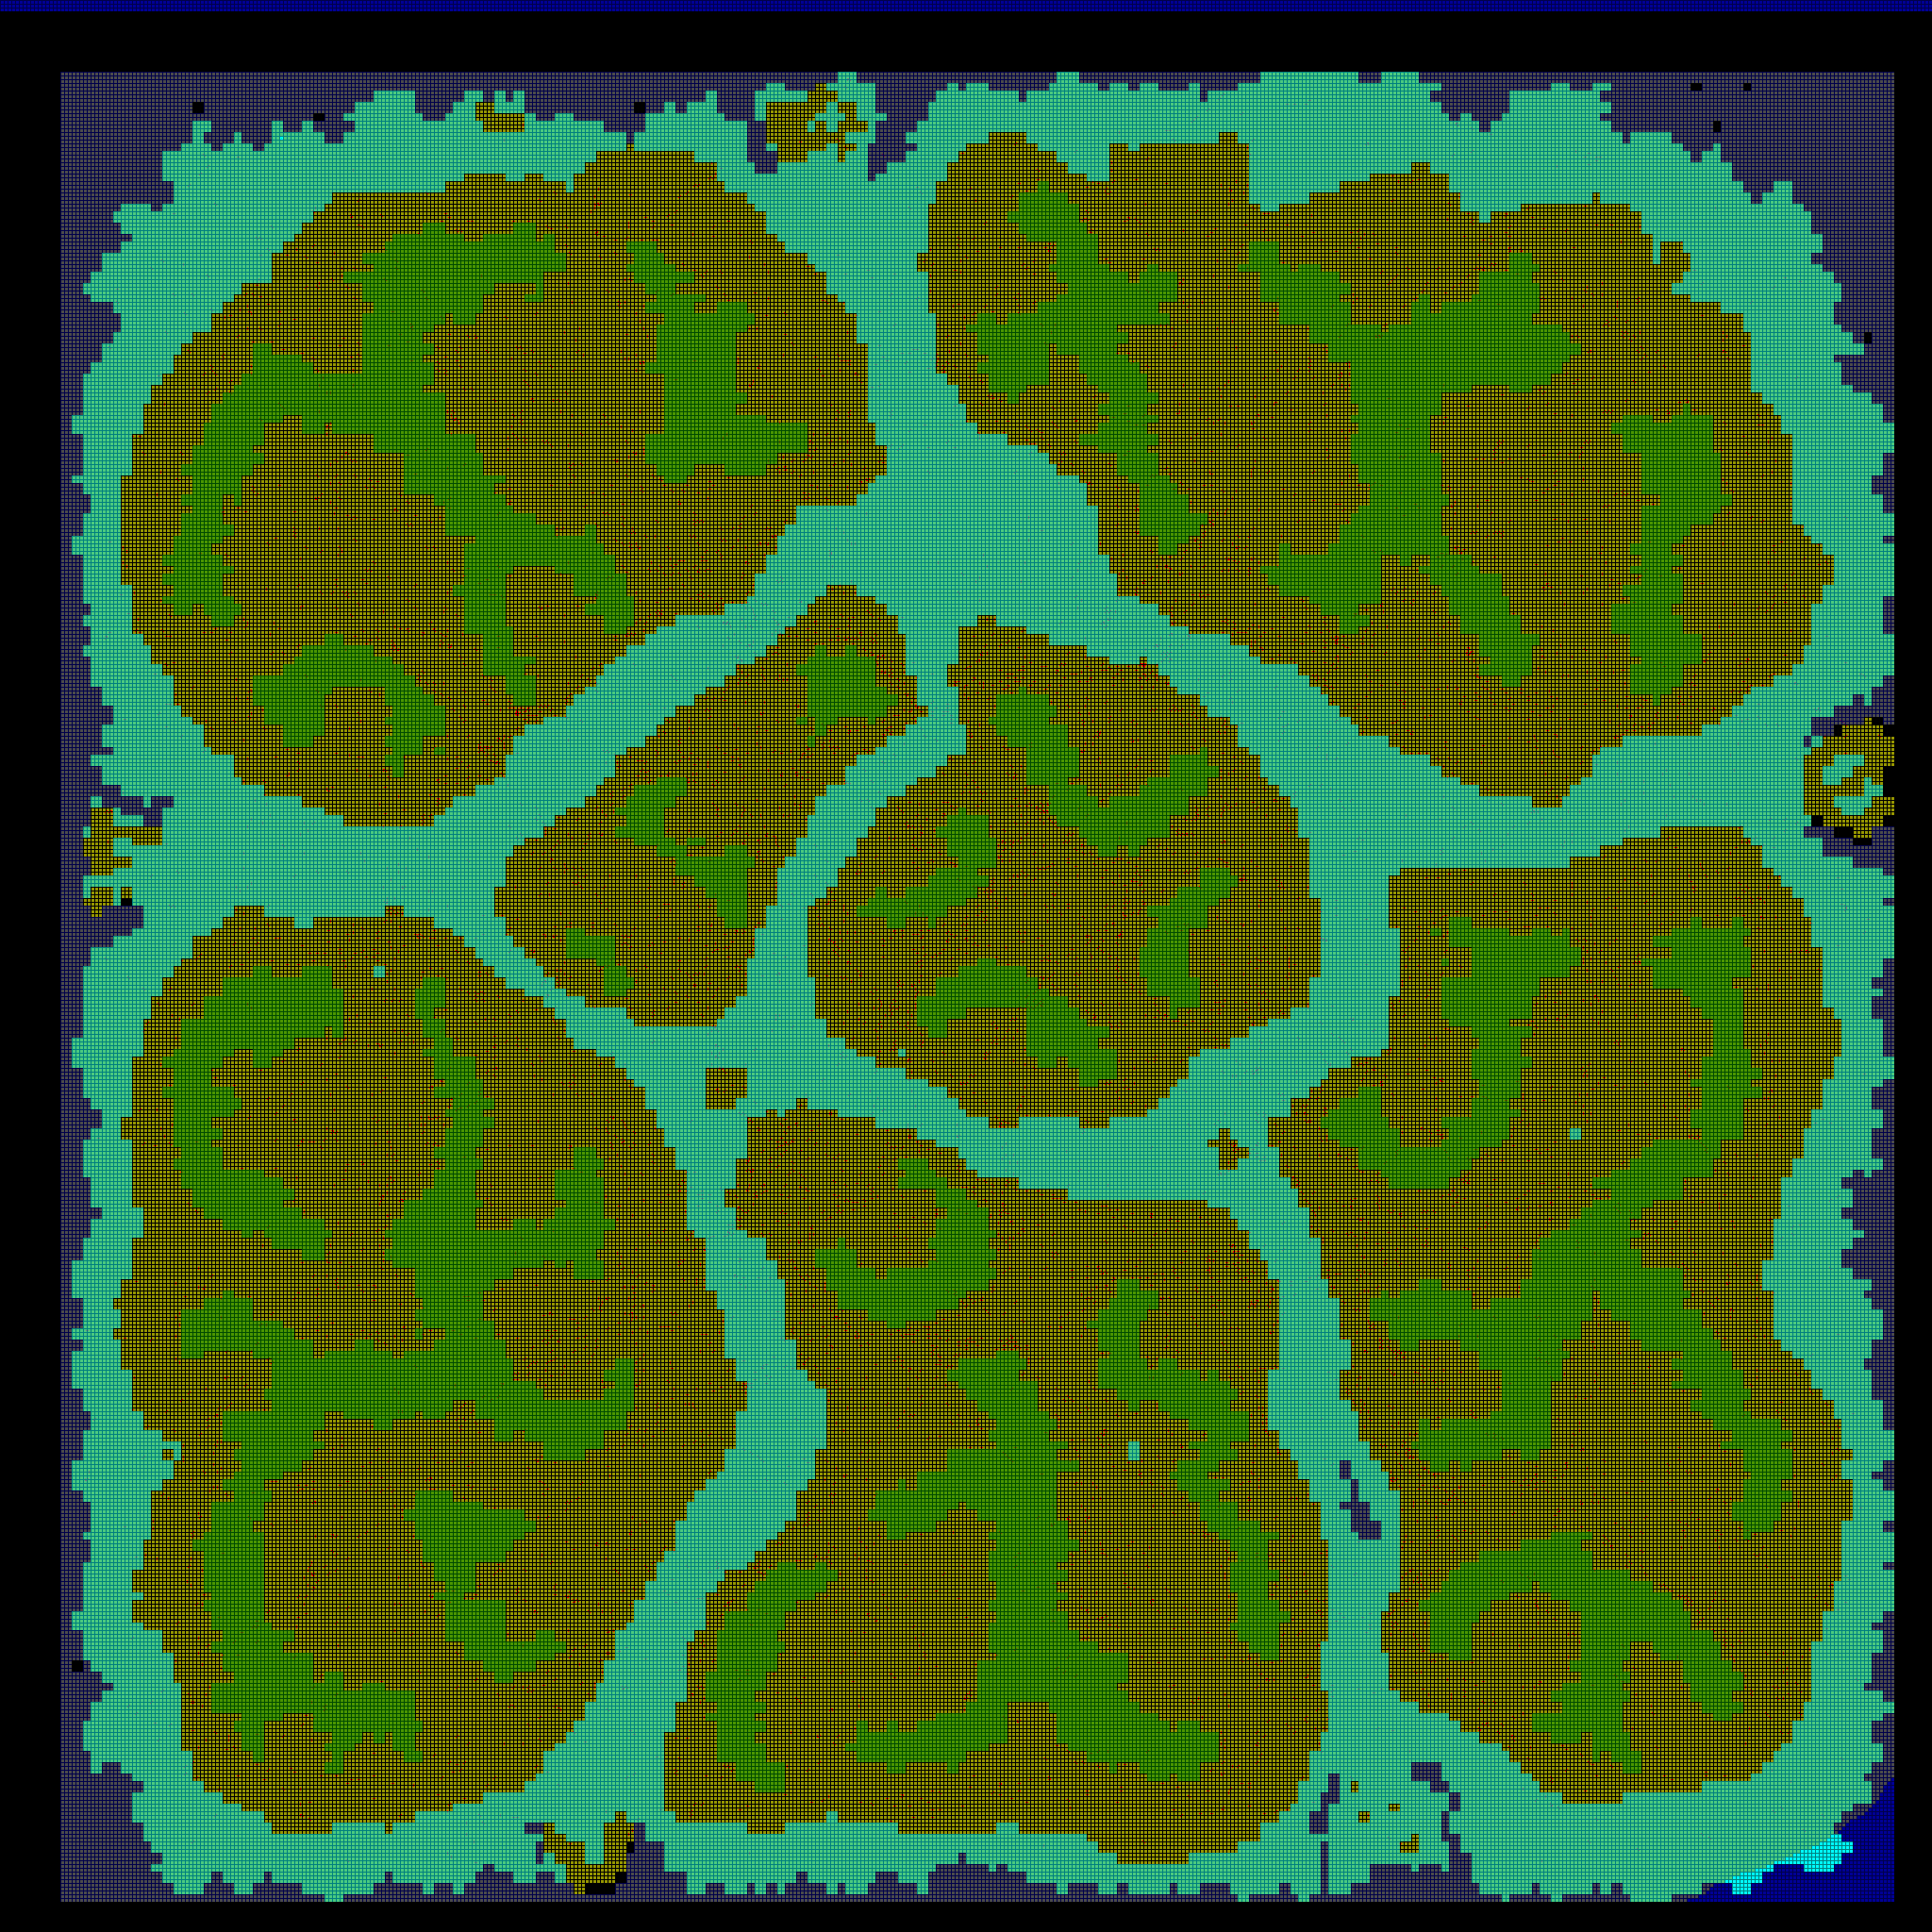
\includegraphics[width=0.8\textwidth]{dijkstra}
		\end{subfigure}
	\end{figure}
\end{frame}

\subsection{}
\begin{frame}{Preliminary Experiment result}
	\begin{figure}
		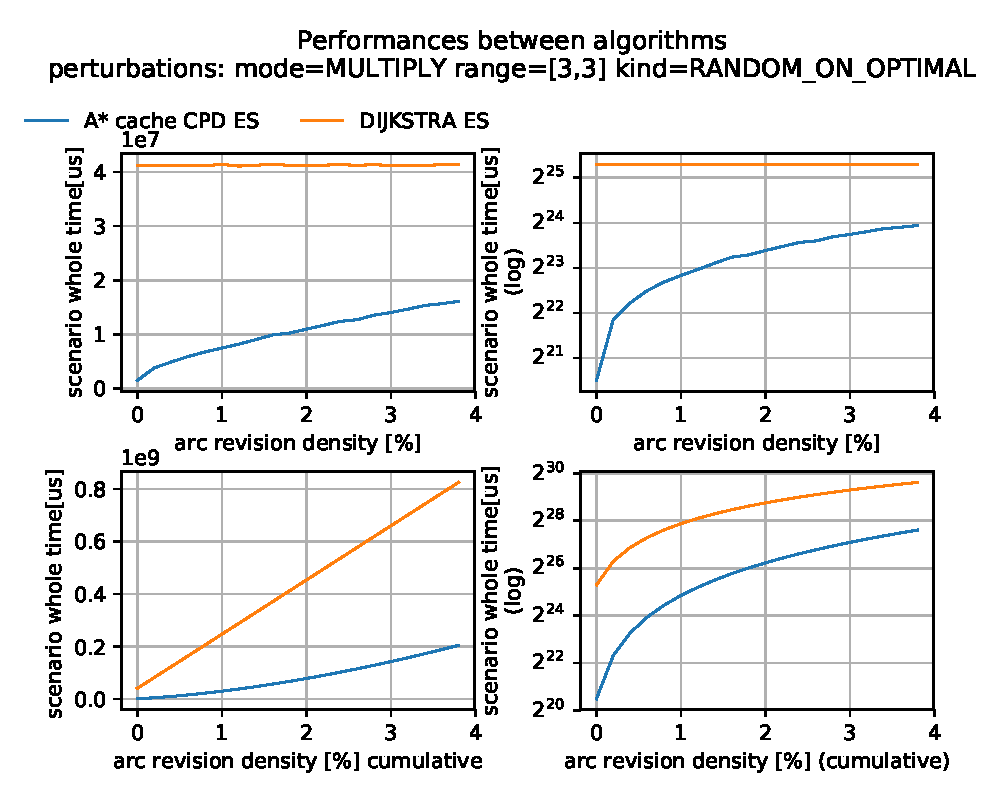
\includegraphics[width=0.8\textwidth]{pathPlanningComparison}
	\end{figure}
\end{frame}

\section{Conclusion and Future Works}

\subsection{}
\begin{frame}{Conclusion and Future Works}
	\begin{itemize}
		\item Introduced Decremental Consistency Checking Problem for Temporal Constraints;
		\item Proposed and experimentally evaluated decremental algorithms for CSPs over PA and Ord-Horn: significant performance gain;
		\item Implemented an algorithm for repairing the optimal path when temporary perturbations occur;
		\item Preliminary results are encouraging;
		\item \textbf{Future works}: dealing with computing the minimal set of constraint relaxation making consistent an inconsistent CSP over PA; Investigate the A* algorithm by setting up more further tests.
	\end{itemize}
\end{frame}


%THANK YOU SLIDE

\usebackgroundtemplate{%
	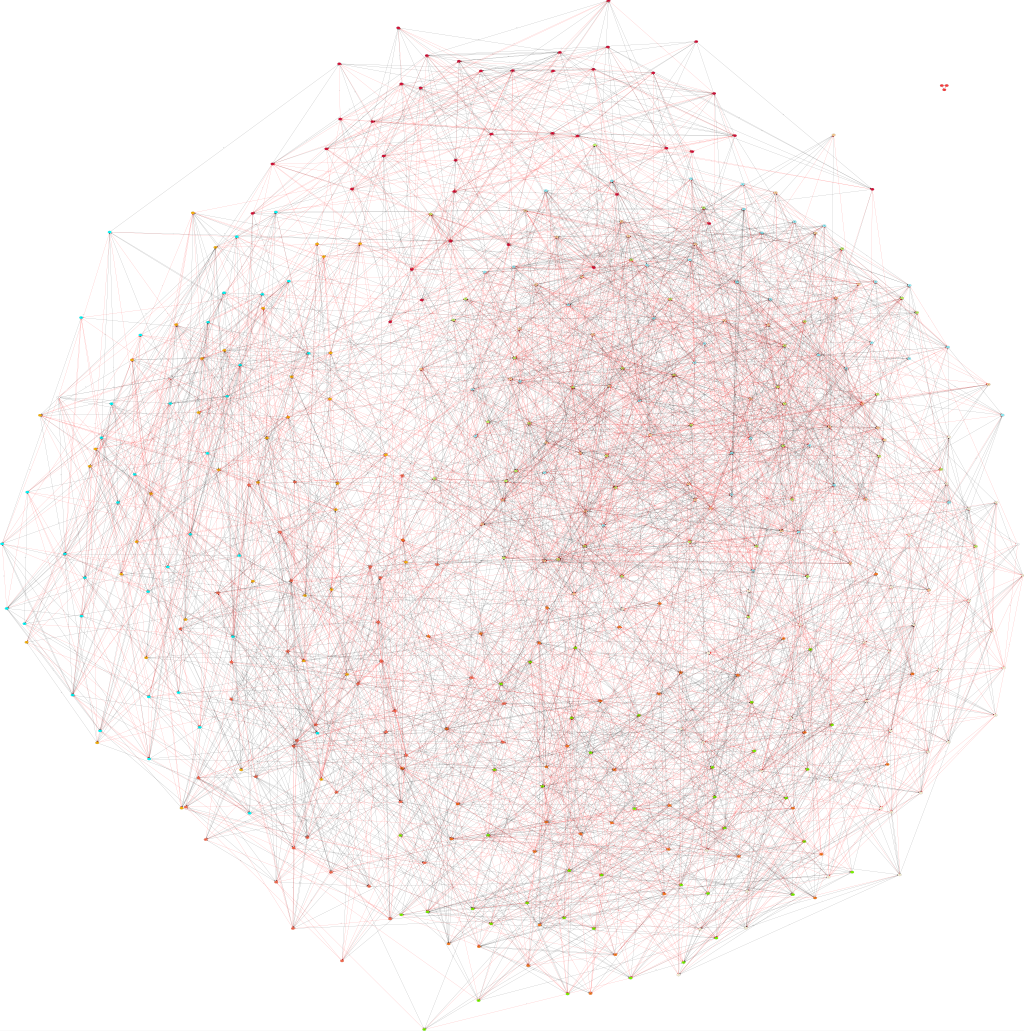
\includegraphics[width=\paperwidth,height=\paperheight]{403}%
}
\setbeamertemplate{footline}{}  
\begin{frame}[plain]
\centering \Huge \textbf{Thanks for listening!\\Any questions???}
\end{frame}

\end{document}